\section{Realisierung}
Nach der vorangegangenen Behandlung der theoretischen Aspekte, sowie der Konzeption des Schalters, erfolgt nun die technische Umsetzung. Dabei wird analog zur Konzeption vorgegangen. 
\subsection{Hardware}
\subsubsection{Raspberry Pi und Schaltung}
Die Realisierung der Schaltung lässt sich in Abbildung \ref{konzeption:schaltplan} nach vollziehen. Es ist gut zu erkennen, dass keine Pull-Up-Widerstände verbaut wurden, da diese intern im Raspberry-Pi vorliegen. Um den Schaltplan auch in der Realität umzusetzen müssen gelötet werden. Jeder Schalter benötigt dazu zwei Kontakte, zum einen seine Signalleitung und zum andern die gemeinsame Masse. Alle Kabel werden zu einem Bus zusammen gelegt und in einem Schrumpfschlauch fixiert, dieser läuft dann zum Raspberry Pi wo die Kabel an die GPIO-Anschlüsse gesteckt werden.   
\begin{figure}[h!tbp]
	\centering
	%hier war leider hässliches Trimming nötig um den Rand des Bildes zu entfernen, da Inkscape Probleme mit dem Export des Schaltplans hatte
	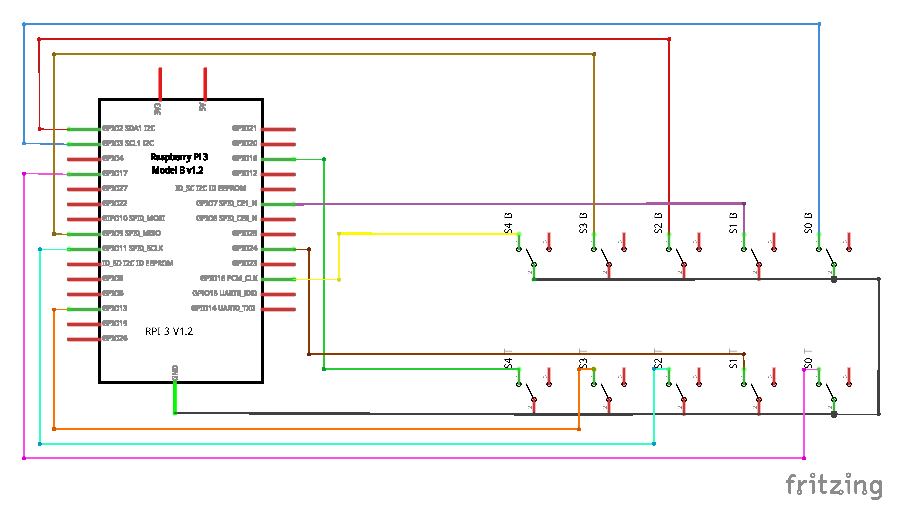
\includegraphics[trim={0.4cm 1cm  0.4cm 0.3cm},clip,width=\textwidth]{bilder/raspi_schaltplan}
	\caption{Schaltplan Fußschalter - ohne Pull-Up-Widerstände, erstellt mit Fritzing }
	\label{konzeption:schaltplan}
\end{figure}	

%Warpfigure, damit die Graphik der Platte nicht zu viel Platz weg nimmt --> Text fließt um Bild.
%[7]wird in Kombination mit \vspace{-32pt} zum Feintuning der Positionierung benutzt, da die automatische Lösung von Latex nicht annehmbar war 
\begin{wrapfigure}[7]{R}{0.4\textwidth}
	\centering
	%wird in Kombination mit [7] zum Feintuning der Positionierung benutzt, da die automatische Lösung von Latex nicht annehmbar war
	\vspace{-32pt}
	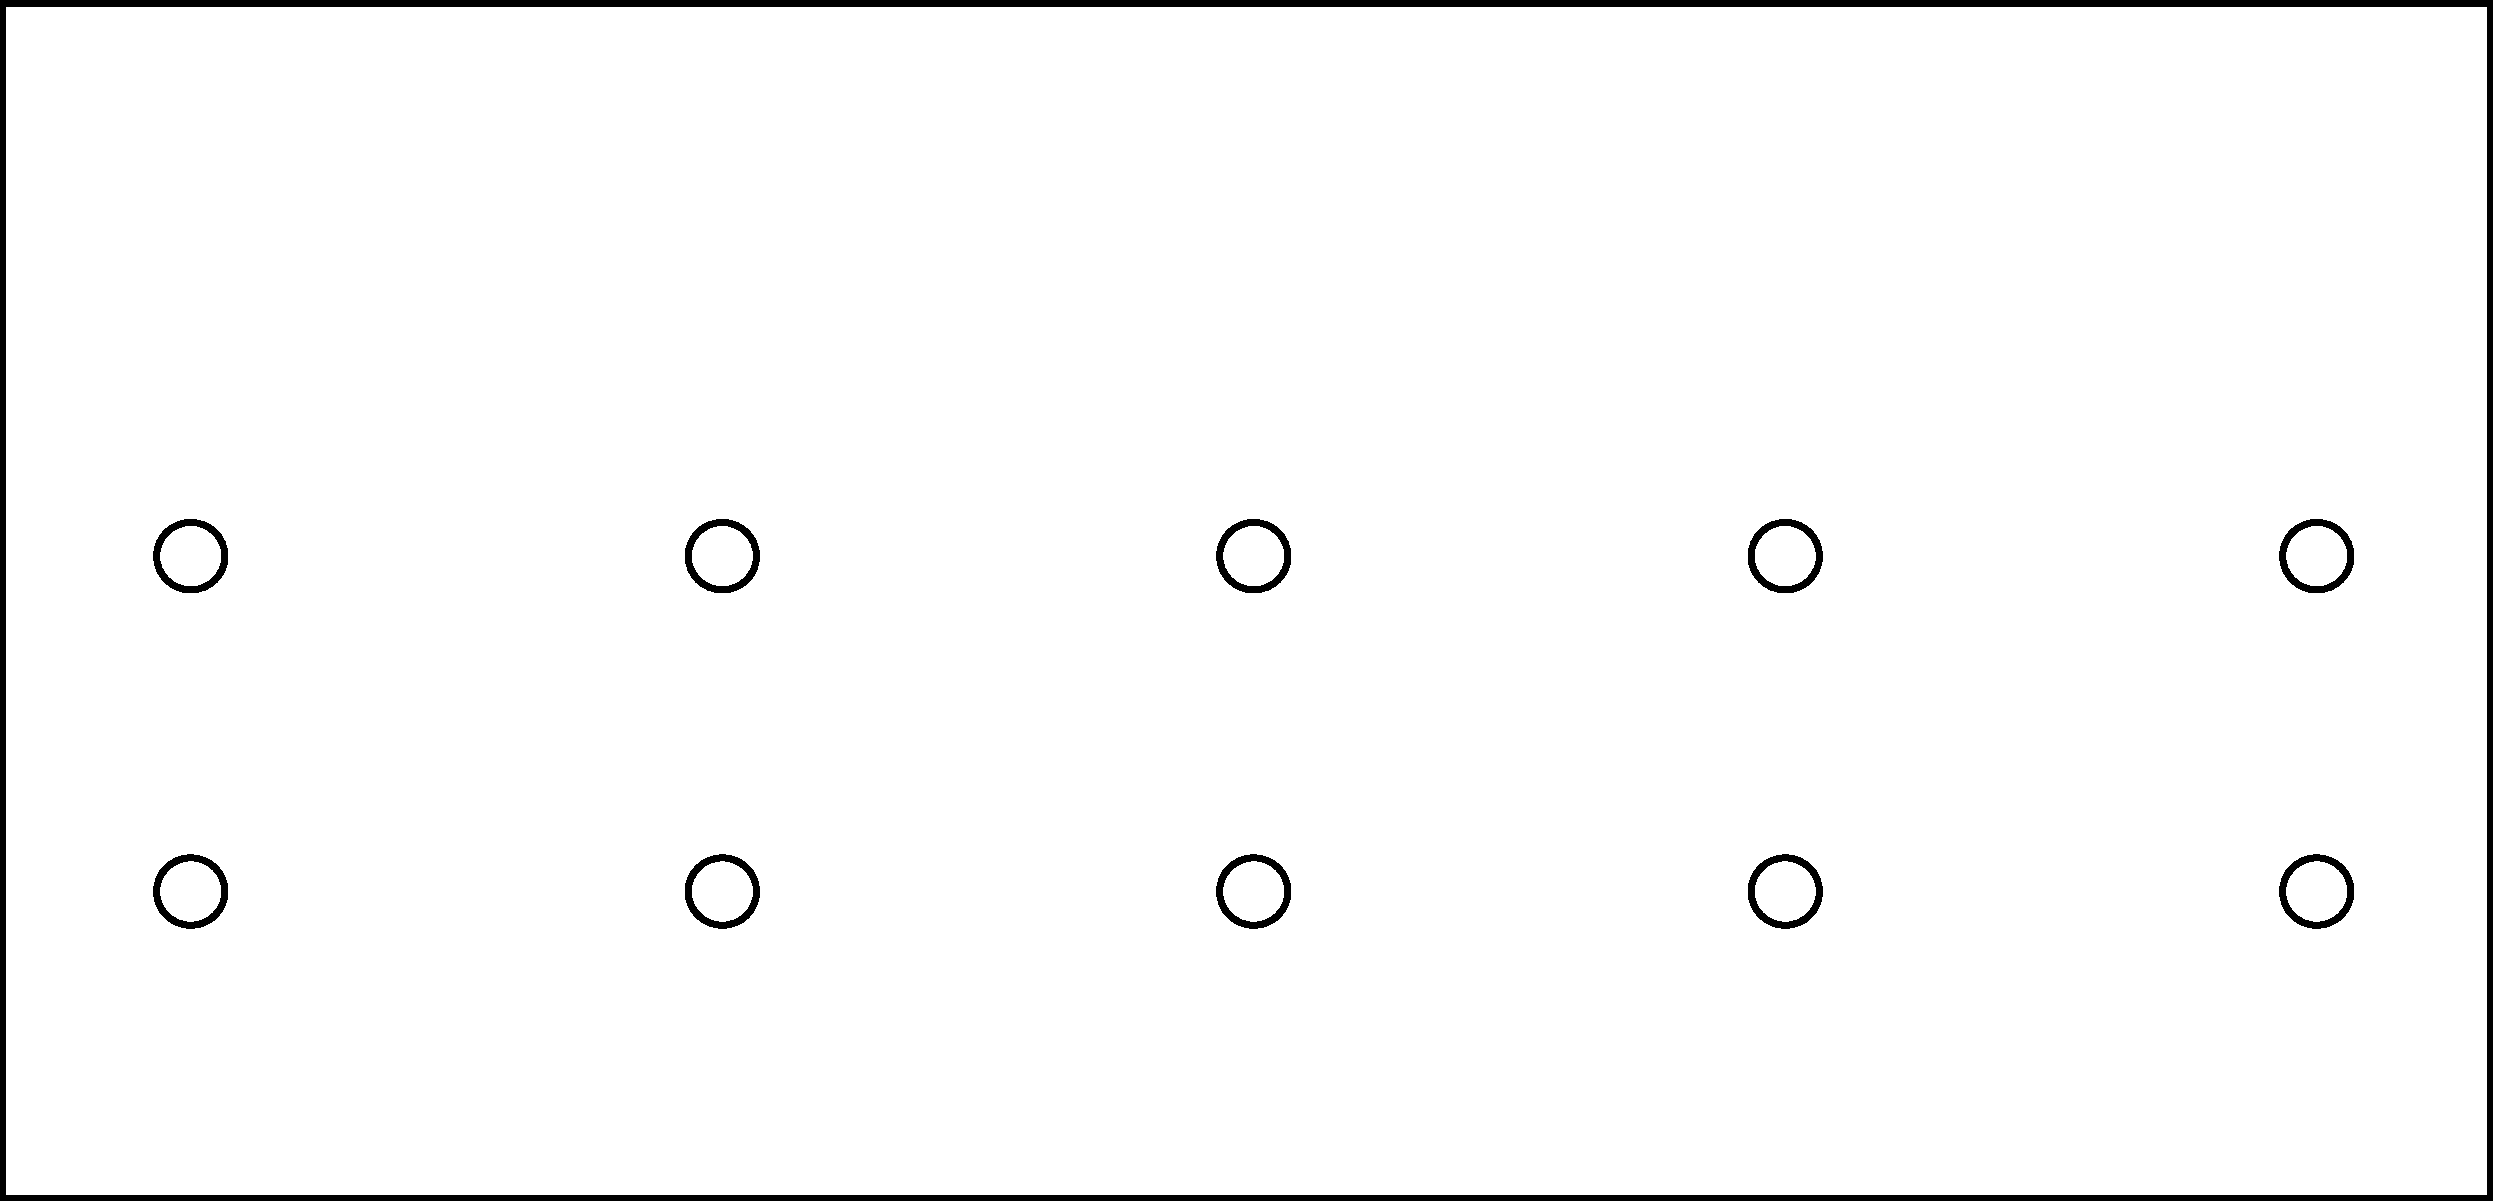
\includegraphics[width=0.4\textwidth]{bilder/svg-schalter}
	\caption{Platte für Fußschalter}
	\label{durchfuehrung:svg-gehause}
\end{wrapfigure}
\subsubsection{Gehäuse Fußschalter}
Für das Gehäuse muss die entsprechende SVG-Datei entworfen werden, damit diese mit einem Laser-Plotter aus einem Stück Acrylglas geschnitten werden kann. In der Abbilung \ref{durchfuehrung:svg-gehause}, ist die Datei dargestellt. Entlang der schwarzen Linien wird geschnitten, sodass die Löcher für die Fußschalter entstehen.
\subsection{Software}
Aus den Recherchen aus Kapitel \ref{chap:theorieundrecherche} sowie der Konzeption in Kapitel \ref{konzeption} haben sich klare Anforderungen an die Software ergeben. Diese gilt es nun umzusetzen. Der folgende Abschnitt wird auf die Anwendungsfälle und notwendigen Schnittstellen eingehen und anhand von Quellcode-Beispielen aufzeigen wie die Konzeption umgesetzt wurde. 
\subsubsection{Schalter und GPIO}
Der Code in Datei \ref{durchfuehrung:gpio} ist stark vereinfacht, doch ist er geeignet um nachzuvollziehen, wie die Schalter ins Programm eingebunden werden. Zunächst muss das GPIO-Modul des Raspberry Pi aufgesetzt werden. Dies geschieht in der ersten Zeile. In der dritten Zeile wird der Pin 17 konfiguriert. Er wird als Input-Pin angemeldet. Mit der Übergabe von \lstinline[language=mypython]{pull_up_down=GPIO.PUD_UP} wird für den Pin der interne Pull-Up-Widerstand aktiviert. 
In der vierten Zeile folgt die Anmeldung des Interrupts. Dieser achtet durch  \lstinline[language=mypython]{GPIO.BOTH} sowohl auf steigende und fallende Flanken. Dadurch funktionieren die Schalter als Taster. Die Entprellzeit wird auf 300\si{ms} eingestellt. Der entscheidende Punkt ist jedoch die Festlegung der Funktion, welche beim Auftreten des Interrupts ausgelöst wird. In den Zeilen fünf und sechs erfolgt schließlich die Definition der Funktion. Sie lädt aus den aktuellen Funktionen die für den Schalter T0 und übergibt sie an die MIDI-Klasse.
%Inkludieren des eines Python-Quellcode, mit Rahmen und dem zuvor Definierten Highlighting 'mypython'
\lstinputlisting[language=mypython,frame=single,caption={Vereinachter Python-Quellcode für GPIO},label={durchfuehrung:gpio}]{code/gpio.py}
\subsubsection{Konfiguration}
Zum Einlesen der Konfigurationsdateien wird die Klasse xmlReader erstellt. Sie benutzt das ElementTree Modul aus Abschnitt \ref{theorie:et}. Außerdem wird die Klasse für die MIDI-Befehle benötigt. Dies geschieht in den ersten drei Zeilen. Was folgt ist der Konstruktor der Klasse. Dieser wird später aufgerufen um ein Objekt der Klasse zu erstellen. Über den Parameter  \lstinline[language=mypython]{configFile} des Konstruktors erfährt die Klasse auch, welche Datei geöffnet werden soll.
Hauptbestandteil der Klasse ist die Funktion \lstinline[language=mypython]{getSettingOfSwitch()} diese iteriert zunächst durch die entsprechende Datei, hier Datei \ref{durchfuehrung:configXML}, und sucht alle XML-Tags die \emph{Schalter} heißen. Von jedem wird die Nummer überprüft. Entspricht diese der gesuchten Nummer (Zeile 9) werden zunächst alle Presets-Tags gesucht, die entsprechenden Zahlen ausgelesen und der Liste angehängt, welche später den Rückgabewert darstellt. Dies geschieht in den Zeilen 8-16.

Anschließend erfolgt das gleiche Verfahren hinsichtlich der Controller in den Zeilen 17-25, Jedoch mit einem Unterschied. In den Controller-Tags der XML-Datei stehen zur Konfiguration Wörter. Es werden jedoch, wie in Abschnitt \ref{konzeption:konfiguration} beschreiben, die entsprechenden Zahlen benötigt um diese via MIDI zu versenden. Aus diesem Grund erfolgt für die Controller noch eine Auflösung der Wörter über die Funktion \lstinline[language=mypython]{midi.setting_resolver}, welcher der Name des Controllers übergeben wird. Diese kann nun zwei verschiedene Werte zurückliefern. Entweder eine Liste aus zwei Einträgen oder eine Liste mit nur einem Eintrag. Letzteres bedeutet, dass sich in der Datei noch ein Parameter befindet. Dieser wird dann schließlich auch ausgelesen, so dass auch für diesen Fall eine Liste mit zwei Einträgen, oder als MIDI-Befehl betrachtet, mit zwei Datenbytes entsteht. Dies wird ebenfalls an den Rückgabewert angehängt.
 
Von dieser Klasse werden beim Start des Hauptprogramms acht Instanzen gebildet, für jede Bank eine. Auf diese Weise können alle Funktionen in das Programm geladen werden und je nach Bank beim Tritt auf einen Schalter an die MIDI-Klasse Übergeben werden.
%Inkludieren des eines Python-Quellcode, mit Rahmen und dem zuvor Definierten Highlighting 'mypython'  
\lstinputlisting[language=mypython,frame=single,caption={Python-Quellcode für Konfiguration GPIO},label={durchfuehrung:config}]{code/config.py}

%Inkludieren des einer XML-Datei, mit Rahmen und dem zuvor Definierten Highlighting 'XML'
\lstinputlisting[language=XML,frame=single,caption={Vereinachte XML-Konfiguration für eine Bank},label={durchfuehrung:configXML}]{code/config.xml}
\subsubsection{MIDI-Befehle}
Die Konzeption aus Abschnitt \ref{konzeption:midi} sieht die Erstellung einer MIDI-Klasse vor. Diese wird hier in Datei \ref{durchfuehrung:midi} dargestellt. Dazu wird wie geplant das Paket RTMIDI benutzt. RTMIDI könnte jedes MIDI-Interface verwenden, welches am Raspberry registriert ist. Um das richtige zu identifizieren nimmt die MIDI-Klasse über den Konstruktor einen String entgegen (Zeile 1) und vergleicht diesen mit der Liste der verfügbaren Ports (Zeile 8). Zuvor wird das RTMIDI-Modul in Zeile 3 als MIDI-Ausgang gestartet. Wird der Port gefunden öffnet die Klasse ihn. In diesem Zustand verweilt die Klasse und wartet darauf, dass ihre Funktionen \lstinline[language=mypython]{programChange()} oder \lstinline[language=mypython]{controllerChange()} aufgerufen werden um MIDI-Befehle zu versenden. Letzte wird hier im Quellcodeauszug in den Zeilen 12 bis 16 veranschaulicht. Das versenden von MIDI-Befehlen mit RTMIDI ist nach der Konfiguration in der vorangegangen Zeilen recht einfach. Aus der Theorie in Abschnitt \ref{theorie:midi} ist bekannt, dass ein MIDI-Befehl drei Bytes besteht. Entsprechend wird hier der Funktion \lstinline[language=mypython]{send_message()} eine Liste von drei Zahlen übergeben. Die erste Zahl wird von der Klasse selber zusammen gestellt. Dabei beinhaltet sie den MIDI-Channel und den Typ der Nachricht, hier hexadezimal \lstinline[language=mypython]{0xB0} also Controller-Change. Die Werte für die Datenbytes ergeben sich als Parameter beim Funktionsaufruf. Analog erfolgt die gleiche Prozedur beim Aufruf der Funktion \lstinline[language=mypython]{programChange}, jedoch mit dem Unterschied dass hier nur Datenbyte übergeben wird.  

Neben den hier dargestellten Funktionen beinhaltet die MIDI-Klasse noch ein Wörterbuch. Mit diesem können die Wörter aus der Konfiguration in MIDI-Befehle umgesetzt werden, wie es in Zeile 18 der Datei \ref{durchfuehrung:config} passiert.
%Inkludieren des eines Python-Quellcode, mit Rahmen und dem zuvor Definierten Highlighting 'mypython'
\lstinputlisting[language=mypython,frame=single,caption={Python-Quellcode zum Initiieren der MIDI-Befehle},label={durchfuehrung:midi}]{code/midi.py} 
